\documentclass{article}

\usepackage{amssymb}
\usepackage{natbib}   
\usepackage{subcaption}
\usepackage{graphicx}
\usepackage{tabularx}
\usepackage{multirow}
\usepackage{adjustbox}
\usepackage[capposition=top]{floatrow}     
\usepackage{booktabs,fixltx2e}      
\usepackage{csvsimple}
\usepackage{longtable}
\usepackage{lscape}
\usepackage[utf8]{inputenc}
\usepackage[font=large,labelfont=bf]{caption}
\usepackage{dcolumn}
\usepackage{float} 
\usepackage{longtable}





\title{Handbook Chapter distributions}
\newcommand{\footremember}[2]{%
    \footnote{#2}
    \newcounter{#1}
    \setcounter{#1}{\value{footnote}}%
}
\newcommand{\footrecall}[1]{%
    \footnotemark[\value{#1}]%
} 
\author{%
  Christian Schuster, Daniel Rogger, Annabelle Wittels, and Robert Lipinski\footremember{trailer}{Rogger (drogger@worldbank.org), Wittels (awittels@worldbank.org) and Lipinski (rlipinski@worldbank.org): Development Impact Evaluation Research Group, The World Bank; Schuster (c.schuster@ucl.ac.uk): University College London. We are grateful to XXX for helpful comments. The findings, interpretations, and conclusions expressed in this paper are entirely those of the authors. They do not necessarily represent the views of the World Bank and its affiliated organizations, or those of the Executive Directors of the World Bank or the governments they represent.}%
 }
\date{February 2021}      % Deleting this command produces today's date.






\begin{document}

\maketitle

\section{Introduction}
\subsection{What are the most common indicators}


\section{Where does the variation lie?}


\subsection{Regression analysis: FE models}


% Table created by stargazer v.5.2.2 by Marek Hlavac, Harvard University. E-mail: hlavac at fas.harvard.edu
% Date and time: Fri, Feb 19, 2021 - 08:52:31
% Requires LaTeX packages: dcolumn 
\begin{table}[!htbp] \centering 
  \caption{FE models - Romania 2019} 
  \label{} 
 \scalebox{0.65}{%
{\small %
\begin{tabular}{@{\extracolsep{5pt}}lD{.}{.}{-3} D{.}{.}{-3} } 
\\[-1.8ex]\hline 
\hline \\[-1.8ex] 
 & \multicolumn{2}{c}{\textit{Dependent variable:}} \\ 
\cline{2-3} 
\\[-1.8ex] & \multicolumn{1}{c}{Satisfaction} & \multicolumn{1}{c}{Pay} \\ 
 & \multicolumn{1}{c}{ } & \multicolumn{1}{c}{ } \\ 
\\[-1.8ex] & \multicolumn{1}{c}{(1)} & \multicolumn{1}{c}{(2)}\\ 
\hline \\[-1.8ex] 
 instAGENTIANATIONALADEADMINISTRAREFISCALA & 9.528 & 3.048^{**} \\ 
  & (7.590) & (1.410) \\ 
  instAGENTIANATIONALAPENTRUZOOTEHNIE & 3.299 & 1.611 \\ 
  & (2.095) & (2.409) \\ 
  instAPIAAGENTIADEPLATISIINTERVENTIEPENTRUAGRICULTURA & 18.568^{**} & 21.867^{**} \\ 
  & (7.837) & (8.540) \\ 
  instCONSILIULJUDETEAN & 8.138^{**} & 8.403^{**} \\ 
  & (3.896) & (4.004) \\ 
  instCURTEADECONTURIAROMANIEI & 3.333^{**} & 5.006^{***} \\ 
  & (1.327) & (1.717) \\ 
  instDIRECTIAGENERALADEASISTENTASOCIALASIPROTECTIACOPILULUI & 17.872^{***} & 25.560^{***} \\ 
  & (4.308) & (5.136) \\ 
  instDIRECTIAJUDETEANADESANATATEPUBLICA & 31.166^{***} & 30.807^{***} \\ 
  & (8.269) & (8.530) \\ 
  instDIRECTIAPENTRUAGRICULTURAJUDETEANA & 2.790 & 4.577 \\ 
  & (1.732) & (3.713) \\ 
  instINSPECTIAMUNCII & 12.856 & 11.467 \\ 
  & (10.837) & (10.925) \\ 
  instINSTITUTIAPREFECTULUI & 13.362^{**} & 21.670^{**} \\ 
  & (6.670) & (9.051) \\ 
  instMINISTERULAGRICULTURIISIDEZVOLTARIIRURALE & 18.274 & 18.503 \\ 
  & (16.199) & (16.483) \\ 
  instMINISTERULAPELORSIPADURILOR & 9.327 & 18.087 \\ 
  & (7.949) & (11.158) \\ 
  instMINISTERULDEZVOLTARIIREGIONALESIADMINISTRATIEIPUBLICE & 8.624 & 14.611^{*} \\ 
  & (6.011) & (7.800) \\ 
  instMINISTERULECONOMIEI & 2.546 & 1.229 \\ 
  & (1.835) & (2.214) \\ 
  instMINISTERULEDUCATIEINATIONALE & 9.736 & 17.146 \\ 
  & (7.841) & (11.045) \\ 
  instMINISTERULFINANTELORPUBLICE & 15.984^{**} & 37.105^{***} \\ 
  & (6.262) & (9.255) \\ 
  instMINISTERULFONDURILOREUROPENE & 10.548^{**} & 21.052^{***} \\ 
  & (5.027) & (6.841) \\ 
  instMINISTERULJUSTITIEI & 13.142 & -2.313 \\ 
  & (10.172) & (1.532) \\ 
  instPRIMARIAMUNICIPIULUIALEXANDRIA & 0.637 & 0.158 \\ 
  & (1.724) & (2.290) \\ 
  instPRIMARIAMUNICIPIULUIBRASOV & 24.873 & 5.548^{***} \\ 
  & (19.719) & (2.053) \\ 
  instPRIMARIAMUNICIPIULUICLUJ-NAPOCA & 0.637 & 2.280^{*} \\ 
  & (1.070) & (1.385) \\ 
  instPRIMARIAMUNICIPIULUICRAIOVA & 1.210 & 1.107 \\ 
  & (1.154) & (1.490) \\ 
  instPRIMARIAMUNICIPIULUIDROBETA-TURNUSEVERIN & 2.286^{*} & 3.161^{*} \\ 
  & (1.245) & (1.652) \\ 
  instPRIMARIAMUNICIPIULUIFOCSANI & 14.819 & 15.260 \\ 
  & (15.301) & (15.200) \\ 
  instPRIMARIAMUNICIPIULUIGALATI & 21.894^{**} & 20.843^{**} \\ 
  & (9.826) & (9.580) \\ 
  instPRIMARIAMUNICIPIULUIIASI & 2.362^{*} & 2.542^{*} \\ 
  & (1.216) & (1.538) \\ 
  instPRIMARIAMUNICIPIULUIORADEA & 28.000^{**} & 46.255^{***} \\ 
  & (11.407) & (14.661) \\ 
  instPRIMARIAMUNICIPIULUISFANTU-GHEORGHE & 22.441 & 100.806^{***} \\ 
  & (15.805) & (32.045) \\ 
  instPRIMARIAMUNICIPIULUITARGOVISTE & 21.532^{*} & 48.206^{***} \\ 
  & (11.658) & (17.476) \\ 
  managerNon-manager & 7.843^{***} & 11.245^{***} \\ 
  & (2.825) & (3.607) \\ 
  genderMale & -6.490^{**} & -13.219^{***} \\ 
  & (2.906) & (3.277) \\ 
  as.numeric(age) & -0.488^{**} & -0.285 \\ 
  & (0.205) & (0.210) \\ 
  as.numeric(tenure) & 0.752^{**} & 0.900^{**} \\ 
  & (0.311) & (0.359) \\ 
  Constant & 15.902^{*} & 4.780 \\ 
  & (8.558) & (9.715) \\ 
 \hline \\[-1.8ex] 
Observations & \multicolumn{1}{c}{5,964} & \multicolumn{1}{c}{5,964} \\ 
R$^{2}$ & \multicolumn{1}{c}{0.009} & \multicolumn{1}{c}{0.018} \\ 
Adjusted R$^{2}$ & \multicolumn{1}{c}{0.004} & \multicolumn{1}{c}{0.013} \\ 
\hline 
\hline \\[-1.8ex] 
\textit{Note:}  & \multicolumn{2}{r}{$^{*}$p$<$0.1; $^{**}$p$<$0.05; $^{***}$p$<$0.01} \\ 
\end{tabular} 
}
}
\end{table} 



% Table created by stargazer v.5.2.2 by Marek Hlavac, Harvard University. E-mail: hlavac at fas.harvard.edu
% Date and time: Fri, Feb 19, 2021 - 08:53:28
% Requires LaTeX packages: dcolumn 
\begin{table}[!htbp] \centering 
  \caption{FE models - Romania 2019} 
  \label{} 
\begin{tabular}{@{\extracolsep{5pt}}lD{.}{.}{-3} D{.}{.}{-3} } 
\\[-1.8ex]\hline 
\hline \\[-1.8ex] 
 & \multicolumn{2}{c}{\textit{Dependent variable:}} \\ 
\cline{2-3} 
\\[-1.8ex] & \multicolumn{1}{c}{Satisfaction} & \multicolumn{1}{c}{Pay} \\ 
 & \multicolumn{1}{c}{ } & \multicolumn{1}{c}{ } \\ 
\\[-1.8ex] & \multicolumn{1}{c}{(1)} & \multicolumn{1}{c}{(2)}\\ 
\hline \\[-1.8ex] 
 Constant & 15.902^{*} & 4.780 \\ 
  & (8.558) & (9.715) \\ 
 \hline \\[-1.8ex] 
Country & \multicolumn{1}{c}{No} & \multicolumn{1}{c}{No} \\ 
Year & \multicolumn{1}{c}{No} & \multicolumn{1}{c}{No} \\ 
Inst & \multicolumn{1}{c}{Yes} & \multicolumn{1}{c}{Yes**} \\ 
Rank & \multicolumn{1}{c}{Yes**} & \multicolumn{1}{c}{Yes*} \\ 
Gender & \multicolumn{1}{c}{Yes***} & \multicolumn{1}{c}{Yes***} \\ 
Age & \multicolumn{1}{c}{Yes**} & \multicolumn{1}{c}{Yes} \\ 
Tenure & \multicolumn{1}{c}{Yes***} & \multicolumn{1}{c}{Yes**} \\ 
\hline \\[-1.8ex] 
Observations & \multicolumn{1}{c}{5,964} & \multicolumn{1}{c}{5,964} \\ 
R$^{2}$ & \multicolumn{1}{c}{0.009} & \multicolumn{1}{c}{0.018} \\ 
Adjusted R$^{2}$ & \multicolumn{1}{c}{0.004} & \multicolumn{1}{c}{0.013} \\ 
\hline 
\hline \\[-1.8ex] 
\textit{Note:}  & \multicolumn{2}{r}{$^{*}$p$<$0.1; $^{**}$p$<$0.05; $^{***}$p$<$0.01} \\ 
\end{tabular} 
\end{table} 


\subsection{Data-driven approach: Ridge regression}



\subsection{country level -- compare distributions of indicators across countries}
\subsection{across institutions}
\subsubsection{Across departments within institutions}
\subsection{Managerial vs. non-managerial level}
\subsection{Tenure}
\subsection{Gender}


\section{Variation over time}
\subsection{Similar patterns over time in relation to macro-factors vs. micro-factors}
\item FEVS over time <- across individuals, within the same Qs
    \item All Qs that are the same for all years
    \item All Qs for all organisations that stay the same <- across indiv., within organisations
\item Chile -- 2 years & variation over time <--   "within" individuals
\item Try to repeat these analyses with Australia, UK and/or Canada
\item Diff-in-Diff: to test the effect of macro-level changes; GDP changes/recession; large scale civil service reforms; changes in government; changes in heads of civil service or the equivalent 


\newpage

\section{\textit{Questions}}\\[0.5in]

\begin{itemize}
    \item Do we want to work with aggregate indices or individual questions? Especially for country-level comparison it would be good to have an (almost) exact overlap between the questions so it might be easier if we use individual questions\\
    \item x

\end{itemize}


\clearpage



\newcolumntype{s}{>{\hsize=.17\hsize\centering\arraybackslash}X}
\newcolumntype{b}{>{\hsize=.35\hsize\raggedright\arraybackslash}X}
\newcolumntype{m}{>{\hsize=.6\hsize\raggedright\arraybackslash}X}


\setcounter{table}{0}
\renewcommand{\thetable}{1.\arabic{table}}


\begin{table}[htbp]
 \begin{adjustbox}{minipage=17cm, center}

 \caption{\textbf{Summary table}\\
          \textbf{The table shows summary statistics for overlapping questions}}

\begin{tabularx}{\textwidth}{bmsssss}
  \toprule
    Country & Variable & Mean & Median & SD & Skewness & Kurtosis \\[.1in]
    \midrule
 \textbf{ALL} & Job satisfaction & 3.81 & 4 & 1.06 & -0.93 & 3.36 \\ 
 \textbf{ALL} & Pay satisfaction & 3.57 & 4 & 1.16 & -0.7 & 2.61 \\ 
 \textbf{ALL} & Work recommendation & 3.79 & 4 & 1.09 & -0.86 & 3.15 \\ 
  FEVS (2019) & Job satisfaction & 3.76 & 4 & 1.07 & -0.88 & 3.23 \\ 
  FEVS (2019) & Pay satisfaction & 3.59 & 4 & 1.15 & -0.73 & 2.7 \\ 
  FEVS (2019) & Work recommendation & 3.77 & 4 & 1.09 & -0.84 & 3.1 \\ 
  Romania & Job satisfaction & 4.61 & 5 & 0.65 & -2.09 & 8.89 \\ 
  Romania & Pay satisfaction & 4.22 & 5 & 1.09 & -1.71 & 5.35 \\ 
  Romania & Work recommendation & - & - & - & - & - \\ 
  Chile & Job satisfaction & 4.16 & 4 & 0.87 & -1.23 & 4.81 \\ 
  Chile & Pay satisfaction & 2.79 & 3 & 1.22 & 0.15 & 1.94 \\ 
  Chile & Work recommendation & 3.81 & 4 & 1.08 & -0.86 & 3.21 \\ 
  Chile (Covid) & Job satisfaction & 4.28 & 4 & 0.85 & -1.48 & 5.73 \\ 
  Chile (Covid) & Pay satisfaction & - & - & - & - & - \\ 
  Chile (Covid) & Work recommendation & 3.98 & 4 & 1.02 & -0.99 & 3.63 \\ 
  Colombia & Job satisfaction & 4.41 & 5 & 0.77 & -1.75 & 7.27 \\ 
  Colombia & Pay satisfaction & - & - & - & - & - \\ 
  Colombia & Work recommendation & 4.38 & 5 & 0.8 & -1.64 & 6.56 \\ 
  Guatemala & Job satisfaction & - & - & - & - & - \\ 
  Guatemala & Pay satisfaction & 3.17 & 4 & 1.11 & -0.28 & 1.78 \\ 
  Guatemala & Work recommendation & - & - & - & - & - \\ 
  
  
  \bottomrule
 \end{tabularx}
\smallskip
\end{adjustbox}
\label{table:summary_tab}
\end{table}


\clearpage


\begin{figure}[htbp]
\centering
%\vspace*{-3cm}
\caption{Distribution of responses to:}
\begin{adjustbox}{max width=1.6\linewidth,center}
\begin{subfigure}{1.2\textwidth}
\caption{\large{Job satisfaction question}}
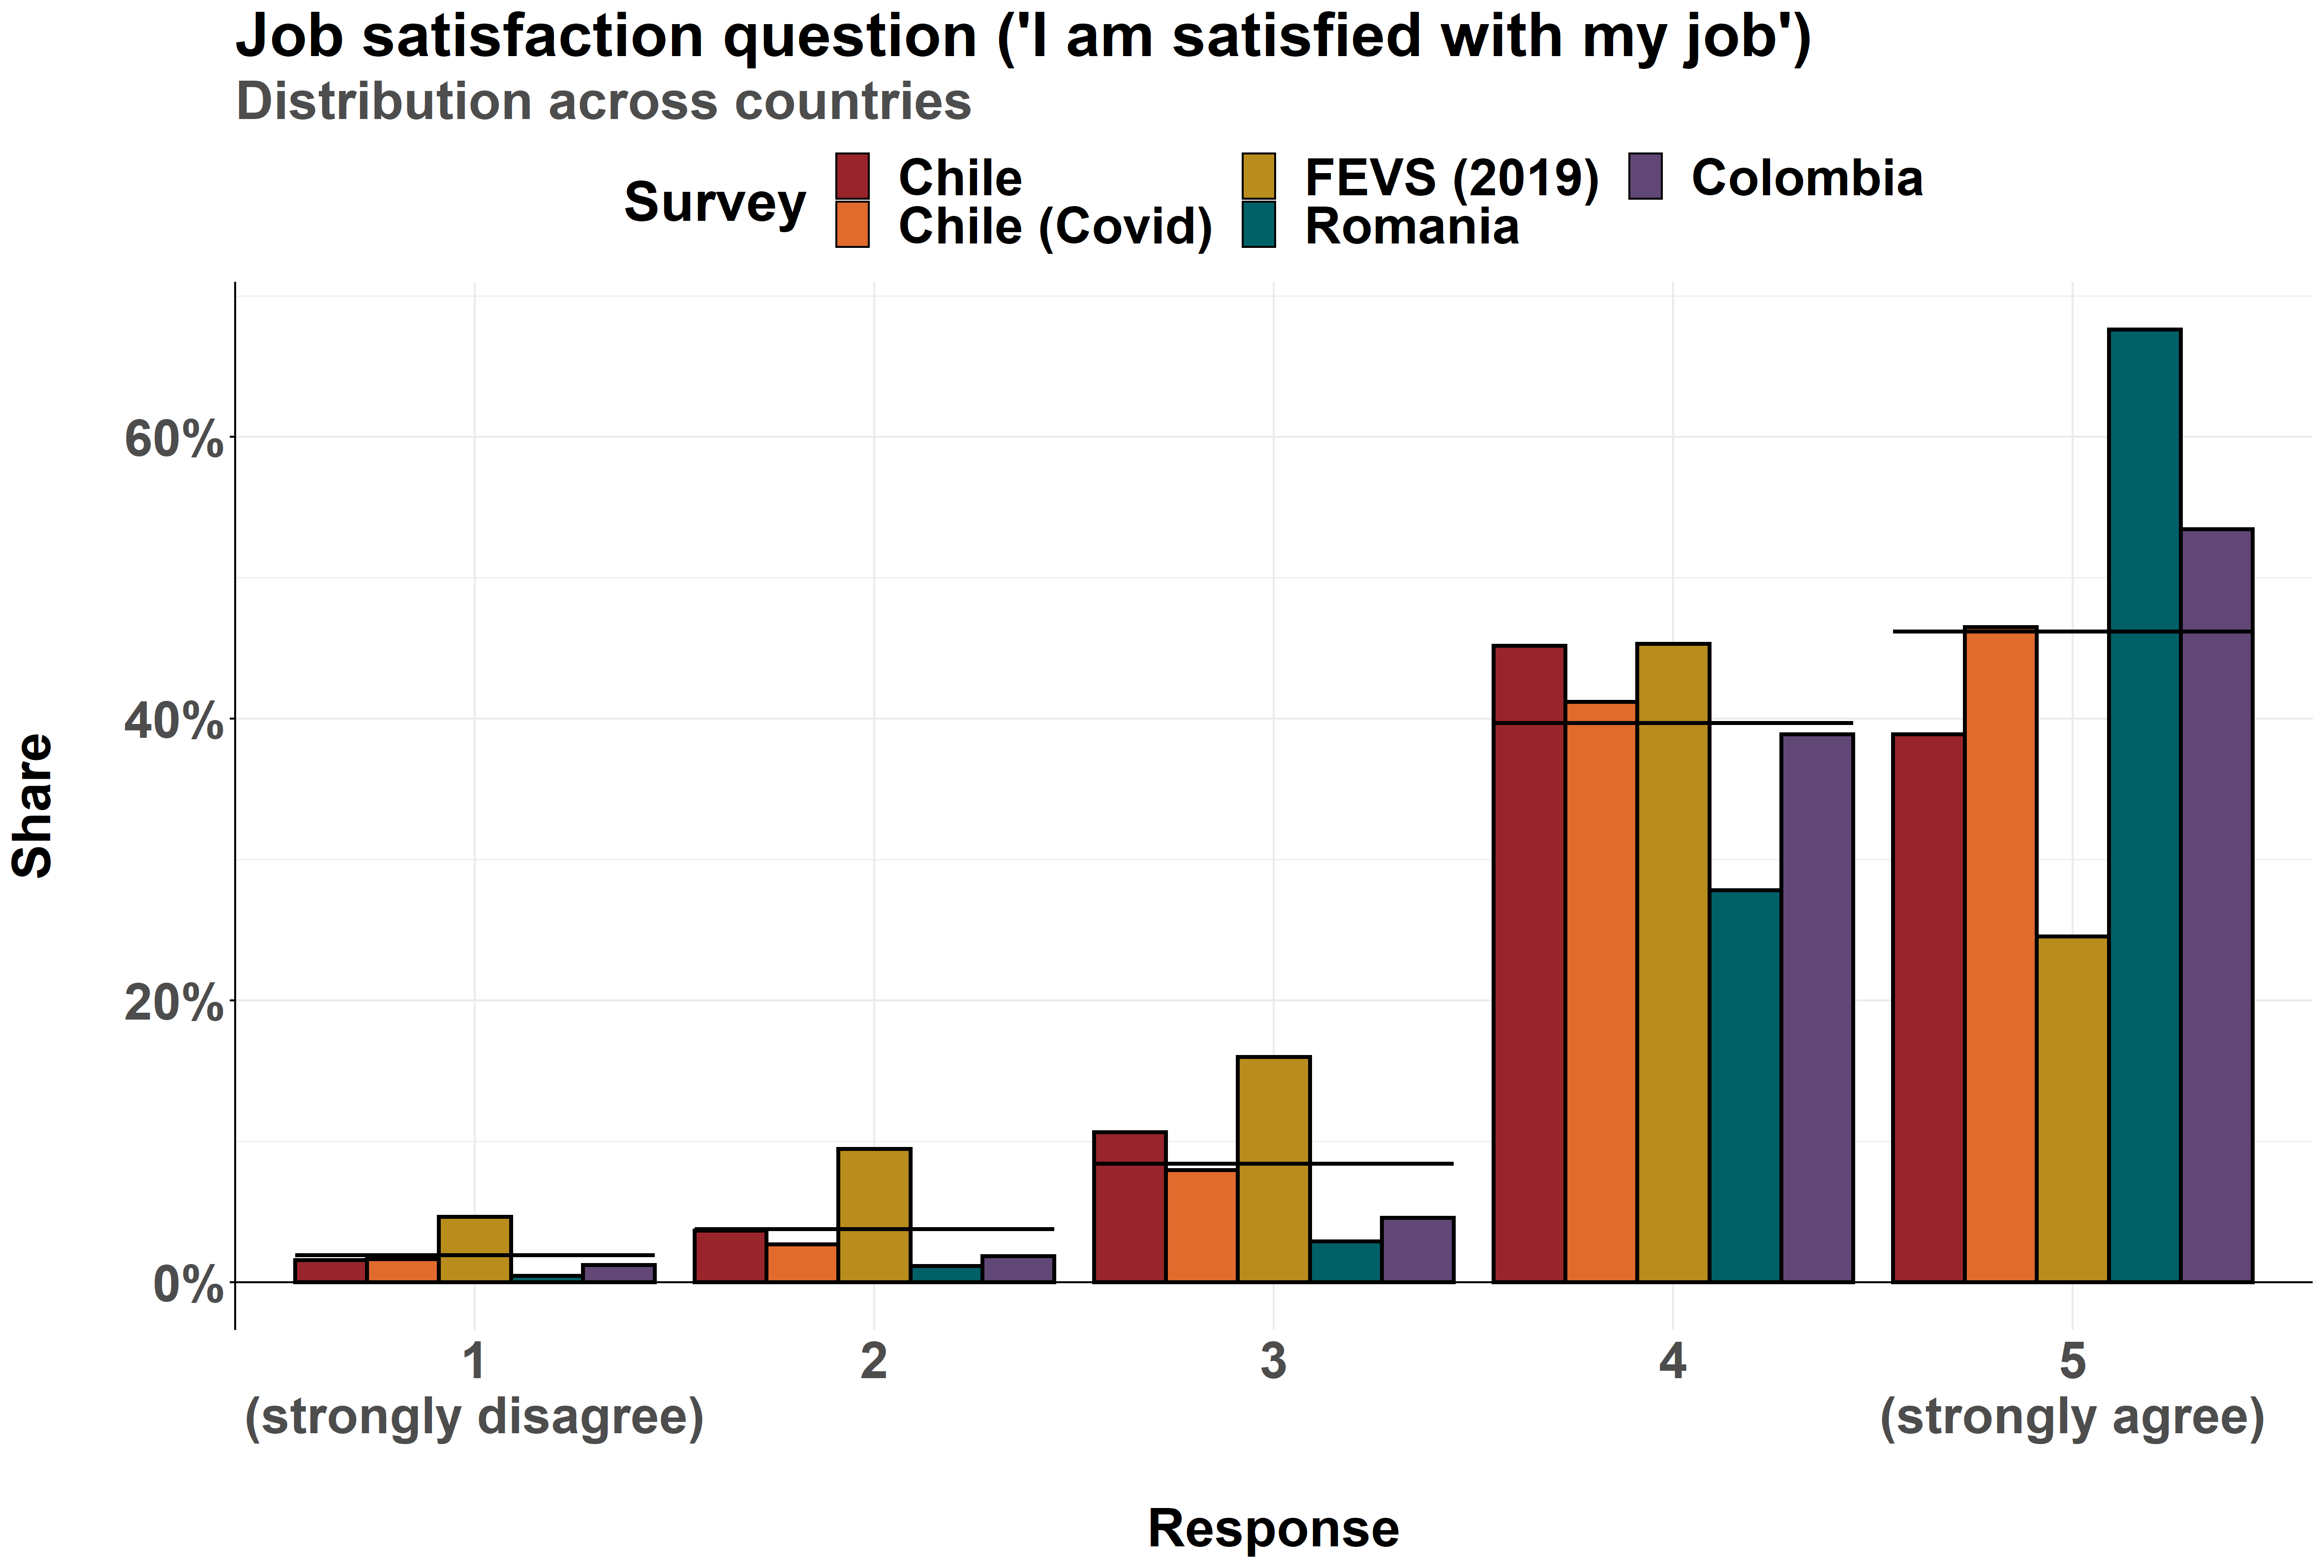
\includegraphics[width= 1\linewidth]{Figures_manual/Variation across countries - satisf_q.png}
\label{fig:dist_satisf_q}
\end{subfigure}
\end{adjustbox}

\hfill

\begin{adjustbox}{max width=1.6\linewidth,center}
\begin{subfigure}{1.2\textwidth}
\caption{\large{Pay satisfaction question}}
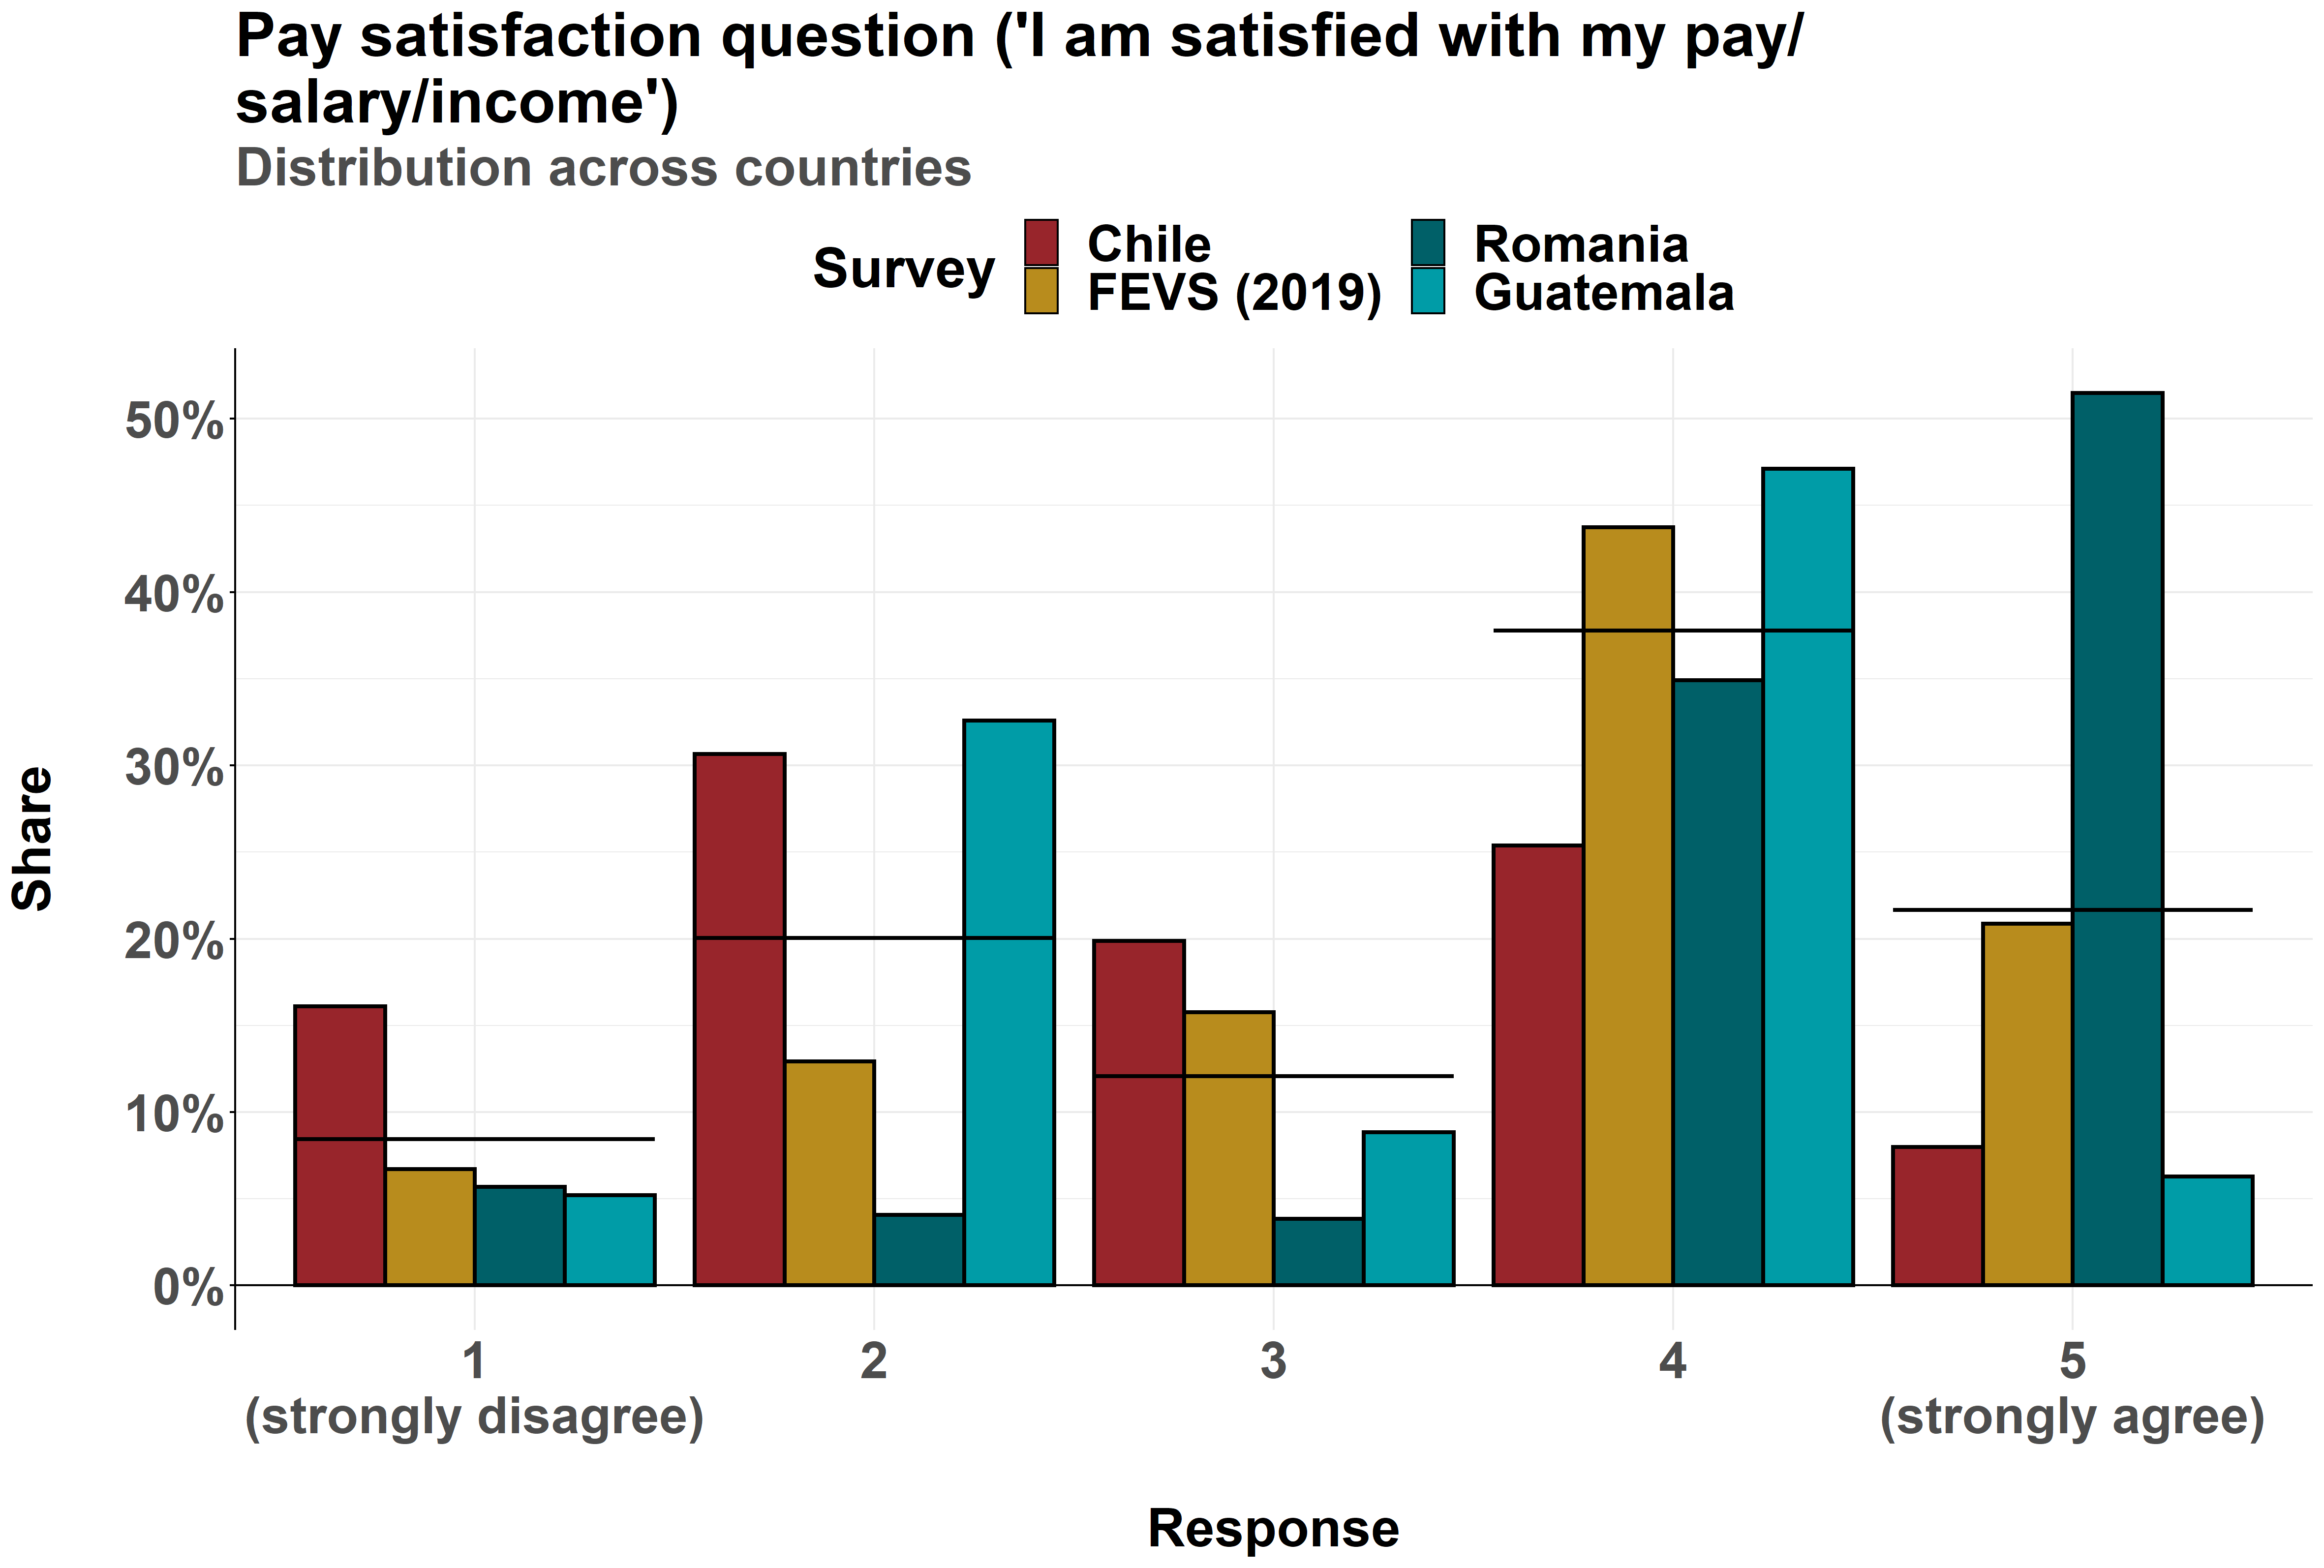
\includegraphics[width= 1\linewidth]{Figures_manual/Variation across countries - pay_satisf_q.png}
\label{fig:dist_pay_satisf_q}
\end{subfigure}

\end{adjustbox}
\label{fig:chile_sample_ci_3}
\end{figure}

\clearpage

\begin{figure}[htbp]\ContinuedFloat
\centering
\begin{adjustbox}{max width=1.6\linewidth,center}
\begin{subfigure}{1.2\textwidth}
\caption{\large{Work recommendation question}}
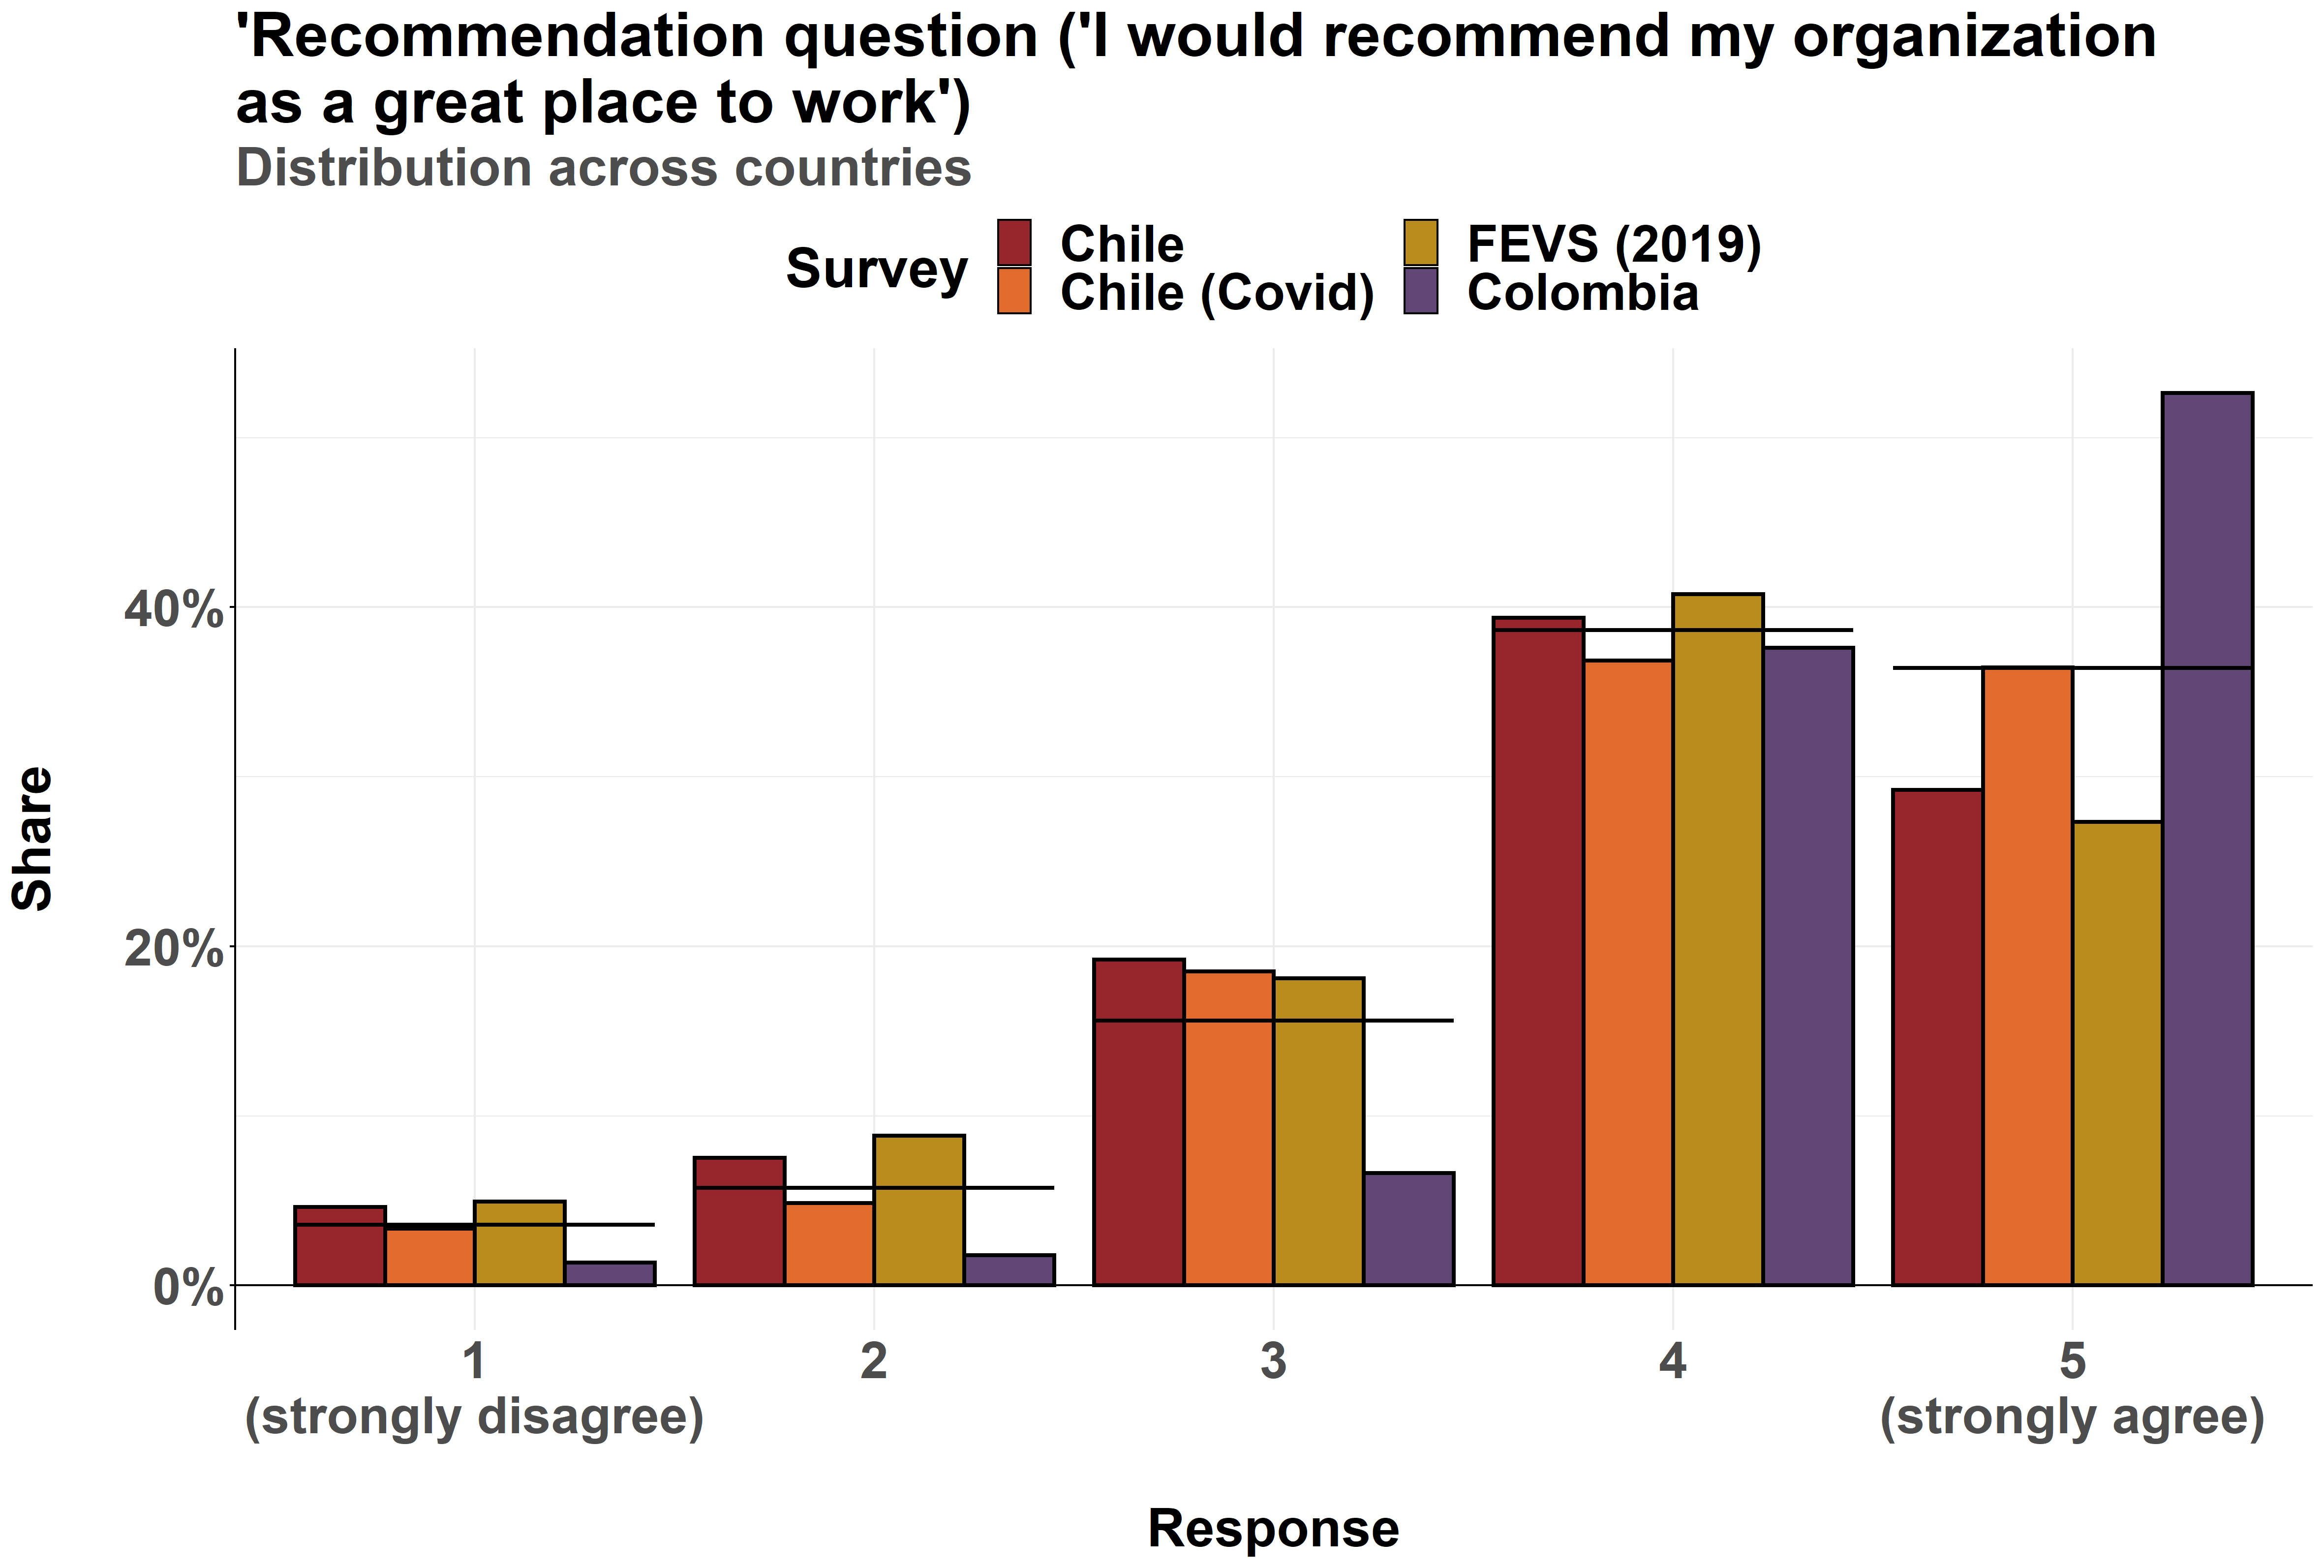
\includegraphics[width= 1\linewidth]{Figures_manual/Variation across countries - recommend_q.png}
\label{fig:dist_recommend_q}
\end{subfigure}

\end{adjustbox}
\label{fig:chile_sample_ci_3}
\end{figure}

\section{Appendix}


\end{document}
